\chapter{Lattice Examples}
\label{c:lat.example}

This chapter gives some examples of how lattice files can be constructred to
describe various machine geometries.

%-----------------------------------------------------------------------------
%%\subsection{Example: Flexible Patch in an ERL}
%%\label{s:ex.erl}
%%
%%\more_\needed
%%
%%Consider the case of an Energy Recovery Linac (ERL) where the beam
%%goes through the linac section of the ERL twice. Once to accelerate
%%the beam and once to decelerate and recover the energy from the
%%beam. The basic ERL lattice is then
%%\begin{example}
%%  erl: line = (injector, merge, linac, arc, linac, dump)
%%  injector: line = (...)
%%  linac: line[multipass] = (..., rf1, ...)
%%  arc: line = (..., patch2)
%%  dump: line = (...)
%%  patch2: patch, flexible = True
%%  ...
%%  expand_lattice
%%  rf1\B2[dphi0] = 0.5
%%  ...
%%\end{example}

%-----------------------------------------------------------------------------
%%\subsection{Example: Injection Line Into a Dipole}
%%\label{s:ex.inj}
%%
%%\begin{figure}[tb]
%%  \centering
%%  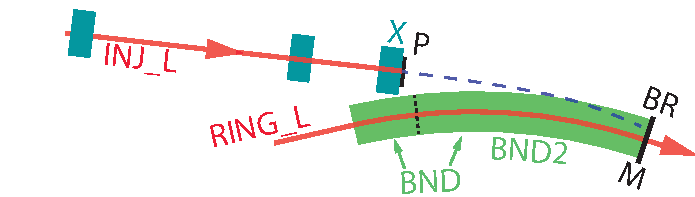
\includegraphics[width=5in]{injection.pdf}
%%  \caption[Injection line into a dipole magnet.]{Injection line into a dipole magnet.}
%%  \label{f:inject}
%%\end{figure}
%%
%%An injection line into a dipole magnet is illustrated in \fig{f:inject}.

%-----------------------------------------------------------------------------
\subsection{Example: Patch Between reversed and non-reversed elements.}
\label{s:ex.patch}

\begin{figure}[tb]
  \centering
  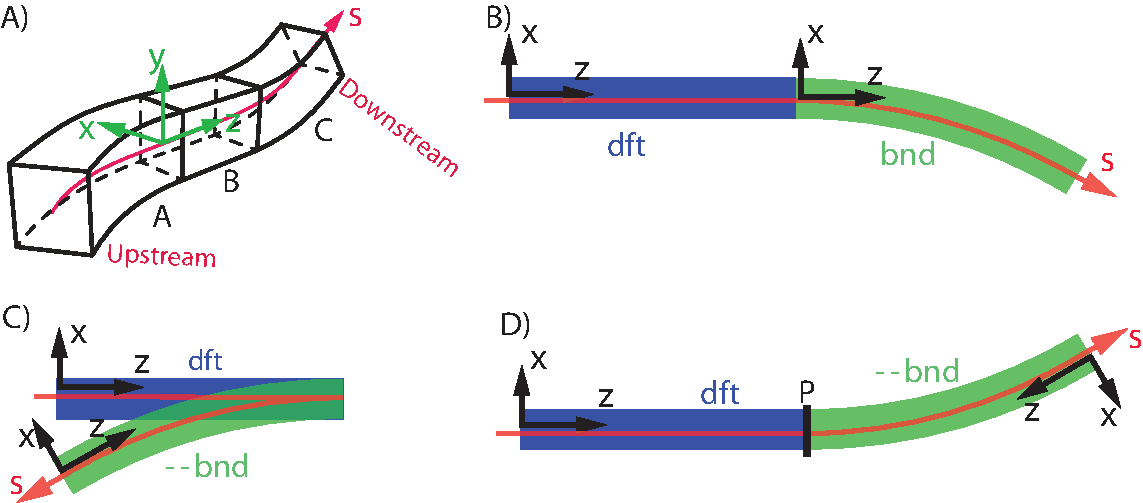
\includegraphics[width=5in]{patch-between.pdf}
  \caption[Patching between reversed and non-reversed elements.]{
Drift element \vn{D} is followed by a reversed drift element \vn{B}.
The view is from $+y$ onto the $x$-$z$ plane. A) If no patch is
present then the geometry does not make physical sense. B) With a
patch in between, a sane geometry can be obtained.}
  \label{f:patch.between}
\end{figure}

\index{patch}
Between normal and reversed elements there must be a reflection
\vn{patch} element (\sref{s:patch}).  This is illustrated in
\fig{f:patch.between}. The basic lattice is
\begin{example}
  D: drift, l = 2
  g_design = pi/12
  B: sbend, l = 2, g = g_design, g_err = -2*g_design
  P: patch, x_pitch = pi
  fig_A: line = (D, --B)     ! Illegal. Do not use!
  fig_B: line = (D, P, --B)  ! Correct
\end{example}
Line \vn{fig_A} represents the situation shown in
\fig{f:patch.between}A.  With no patch between the drift \vn{D} and
the reversed bend \vn{B}, a particle leaving \vn{D} at \vn{D}'s
downstream end will find itself outside of both \vn{D} and
\vn{B}. Clearly this is an unphysical situation. Sanity is restored in
line \vn{fig_B} shown in \fig{f:patch.between}B. In this instance, the
patch \vn{P} rotates the reference coordinates around the $y$-axis
leaving the $y$-axis invariant the bend of \vn{B} is in the $x$-$z$
plane. There are other patch parameter values that could be used to
produce a reflection patch (\sref{s:patch.coords}).  For example,
Setting the patch's \vn{y_pitch} to \vn{pi} would produce a reflection
patch.

Since bend \vn{B} is reversed, A particle moving downstream within
\vn{B} is going the opposite direction from the normal direction. If
\vn{g_err} were zero in this instance, a downstream moving particle
would feel a force that will rotate the particle in a clockwise manner
opposite from the counterclockwise direction of the bend. To counter
this, \vn{g_err} is set so the total bending field \vn{g_tot = g +
g_err} is opposite the design field. That is, \vn{g_err} is set so
that \vn{g_tot = -g}.

%-----------------------------------------------------------------------------
\subsection{Example: Colliding Beam Storage Rings}
\label{s:ex.collide}

\begin{figure}[tb]
  \centering
  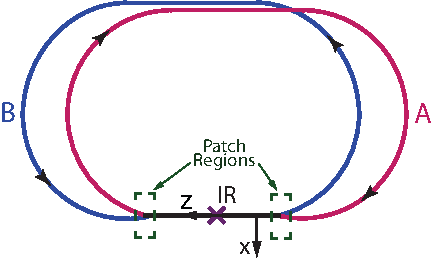
\includegraphics[width=5in]{colliding-beams.pdf}
  \caption[Dual ring colliding beam machine]{Dual ring colliding beam machine. 
The beam in the \vn{A} ring rotates clockwise and in the \vn{B} ring
counterclockwise.}
  \label{f:collide}
\end{figure}

The idealized layout of a pair of storage rings used for colliding
counter rotating beams is shown in \fig{f:collide}. Rings \vn{A} and
\vn{B} intersect at two interaction regions labeled \vn{ir1} and
\vn{ir2} where the beams collide. The basic lattice description is:
\begin{example}
  ir1: line[multipass] = (...)
  ir2: line[multipass] = (...)
  m: marker
  fid: fiducial, origin_ele = m
  ...
  a: line = (arc_a1, pa1_in, ir1, m, pa1_out, arc_a2, pa2_in, ir2, pa2_out)
  b_rev: line = (arc_b1, pb1_in, ir1, fid, pb1_out, arc_b2, pb2_in, ir2, pb2_out)
  b: line = (--b_rev)
  use, a, b
\end{example}
Lines \vn{ir1} and \vn{ir2} are the two interaction regions which are
declared \vn{multipass} since they are shared by the two rings. Line
\vn{a} represents ring \vn{A} where the beam which, by definition,
travels in the same direction as increasing $s$, rotates clockwise.
Line \vn{b_rev} is a ``reversed'' line of ring \vn{B} and, like
\vn{a}, represents a beam rotating clockwise.  Line \vn{b}, which
represents ring \vn{B}, is the reverse of \vn{b_rev} and here the beam
rotates counterclockwise. In this construction, all elements of \vn{b}
are reversed.  While this is not mandatory (only the interaction
regions must be reversed in \vn{b}), having all of \vn{b} reversed
simplifies the geometry since this means that the local coordinate
systems of both lines \vn{a} and \vn{b} will be ``aligned'' with the
$x$-axis pointing to the outside of the ring and the $y$-axis pointing
up, out of the page. Having non-aligned coordinate systems is possible
but potentially very confusing.

The two rings are physically aligned using a marker \vn{m} in \vn{a}
and a \vn{fiducial} element \vn{fid} in \vn{b} that aligns with
\vn{m}.  Each ring has four rigid \vn{patch} elements, whose name
begins with \vn{p}, on either side of each interaction region.

The finished lattice will have two branches, The first branch (with
index 0) will be derived from line \vn{a} and the second branch (with
index 1) will be derived from line \vn{b}. The multipass lords
representing the physical IR elements will be in the ``lord section''
of branch 0. 
